\documentclass{article}

\usepackage{booktabs}
\usepackage{tabularx}
\usepackage{hyperref}
\usepackage{float}
\usepackage{graphicx}
\usepackage{tabularray}
\usepackage{xcolor}

\newcolumntype{L}[1]{>{\RaggedRight\arraybackslash}p{#1}}
\newcolumntype{Y}{>{\RaggedRight\arraybackslash}X}

\hypersetup{
    colorlinks=true,       % false: boxed links; true: colored links
    linkcolor=red,          % color of internal links (change box color with linkbordercolor)
    citecolor=green,        % color of links to bibliography
    filecolor=magenta,      % color of file links
    urlcolor=cyan           % color of external links
}

\title{Hazard Analysis\\\progname}

\author{\authname}

\date{}

%% Comments

\usepackage{color}

\newif\ifcomments\commentstrue %displays comments
%\newif\ifcomments\commentsfalse %so that comments do not display

\ifcomments
\newcommand{\authornote}[3]{\textcolor{#1}{[#3 ---#2]}}
\newcommand{\todo}[1]{\textcolor{red}{[TODO: #1]}}
\else
\newcommand{\authornote}[3]{}
\newcommand{\todo}[1]{}
\fi

\newcommand{\wss}[1]{\authornote{magenta}{SS}{#1}} 
\newcommand{\plt}[1]{\authornote{cyan}{TPLT}{#1}} %For explanation of the template
\newcommand{\an}[1]{\authornote{cyan}{Author}{#1}}

%% Common Parts

\newcommand{\progname}{Software Engineering} % PUT YOUR PROGRAM NAME HERE
\newcommand{\authname}{Team \#18, Gouda Engineers 
\\ Aidan Goodyer
\\ Jeremy Orr
\\ Leo Vugert
\\ Nathan Perry
\\ Tim Pokanai} % AUTHOR NAMES                  

\usepackage{hyperref}
    \hypersetup{colorlinks=true, linkcolor=blue, citecolor=blue, filecolor=blue,
                urlcolor=blue, unicode=false}
    \urlstyle{same}
                                


\begin{document}

\maketitle
\thispagestyle{empty}

~\newpage

\pagenumbering{roman}

\begin{table}[hp]
\caption{Revision History} \label{TblRevisionHistory}
\begin{tabularx}{\textwidth}{llX}
\toprule
\textbf{Date} & \textbf{Developer(s)} & \textbf{Change}\\
\midrule
Date1 & Name(s) & Description of changes\\
Date2 & Name(s) & Description of changes\\
... & ... & ...\\
\bottomrule
\end{tabularx}
\end{table}

~\newpage

\tableofcontents

~\newpage

\pagenumbering{arabic}

\wss{You are free to modify this template.}

\section{Introduction}

Hazard analysis is an important part of this project because it identifies potential risks and outlines how to mitigate and plan for errors that could occur during the development and operating. Conducting this analysis helps ensure that safety, reliability, and stability are addressed early in the design process.

A hazard is a condition in which a failure, malfunction, or unintended behavior of the software occurs which can cause harm, loss, or an unsafe system state.

\section{Scope and Purpose of Hazard Analysis}

The scope of this analysis includes all major software components of the system, such as the data retrieval module interfacing with the FRDR API, the data processing and analysis algorithms, and the user interface for visualization and interaction. External components, including FRDR’s data infrastructure and third-party libraries such as machine learning or natural language processing models. These are considered only in terms of their interactions with the system.

The primary purpose of conducting this analysis is to identify software related hazards that could compromise the accuracy, reliability, or security of the system’s outputs. Potential losses include the generation of misleading behavioural metrics, corruption or misrepresentation of research data, or loss of data availability. By identifying these risks early, this analysis supports the development of safety and security requirements that promote data integrity, consistent functionality, and reliable operation for all users.

\wss{You should say what \textbf{loss} could be incurred because of the hazards.}

\section{System Boundaries and Components}

\wss{Dividing the system into components will help you brainstorm the hazards.
You shouldn't do a full design of the components, just get a feel for the major
ones.  For projects that involve hardware, the components will typically include
each individual piece of hardware.  If your software will have a database, or an
important library, these are also potential components.}

\par{ The components of the system that will be subject to the hazard analysis are as follows:}

\begin{enumerate}
    \item \textbf{The FRDR Database:} All 29 individual datasets and 60,000 relevant data objects that exist on this repository. Note that this component is
    incorporated into the system in a read-only fashion meaning that at no point in the system creation will any part of it be changed, developed or written to
    with the exception of Dr. Henry Szechtman or Dr. Anna Dvorkin-Gheva depositing more data into the repository, the execution of which is seperate from the system.
    \item \textbf{Front-End Query Application:} A front-end web application that provides access for users to query results from the system. This component contains
    some subcomponents
        \begin{itemize}
            \item \textbf{Natural Language Processor:} This subcomponent takes in natural language input and uses an LLM to generate a relevant query.
            \item \textbf{Filter Query Engine:} This subcomponent allows the user to manually add filters based on trial data and generates a relevant query.
            \item \textbf{Webstore Query Engine:} This subcomponent provides pre-defined result sets that may be relevant to the user for the user to browse and
            use if relevant.
        \end{itemize}
    \item \textbf{API Layer:} An API layer will be implemented to connect the constructed system with the FRDR database. This layer will be responsible for 
    retrieving the relevant data from the FRDR for each individual query.
    \item \textbf{Backend System:} This component includes several subcomponents:
        \begin{itemize}
            \item \textbf{Database Schema:} This subcomponent is a database scehma which unifies the datasets into one schema while also connecting the metadata annotations
            and related data objects in the format of a relational DBMS and points to the FRDR database.
            \item \textbf{Behavioural Analysis LLM:} This subcomponent contains the business logic and an LLM model responsible for categorizing the trials
            based on compulsive behaviour or rat poses.
            \item \textbf{Visualization Engine:} This subcomponent is responsible for taking a result set and generating requested visualizations from it.
        \end{itemize}
\end{enumerate}

\section{Critical Assumptions}


\begin{enumerate}
    \item FRDR API Availability
    \item[] It is assumed that the FRDR repository and corresponding API will remain accessibile and availabile throughout the lifetime of the product. API outages and/or other lapses in availability of this resource will be considered outside of the team's control. 
    \item Read-Only Data Access
    \item[] It is assumed that the system will access the FRDR dataset solely in a read-only manner. Therefore, the system will not add, modify, or delete data from the source repository. 
    \item Minimum System Access Standards
    \item[] It is assumed that a user will access the system from a modern browser with JavaScript enabled. 
    \item Source Data Integrity 
    \item [] The system assumes that the individual data objects are accurate and correctly-labeled, therefore the corerrectness of experiments drawn from the platform is independent of the FRDR. 
\end{enumerate}

\section{Failure Mode and Effect Analysis}

\subsection{Hazards Considered Out of Scope}

\begin{itemize}
    \item The FRDR domain goes down for reasons such as maintenance or an outage
    \item The FRDR repository or a subset of it is lost or corrupted
    \item Addition, modification, or deletion of FRDR data by an authorized user
    \item Pre-existing errors in FRDR metadata and mislabeled entries
    \item The user misuses data by making an error in interpreting information through the system's data visualizer
    \item User experience affected by local system issues such as slow internet or failing hardware
\end{itemize}

\subsection{Failure Modes and Effect Analysis Table}

\begin{longtblr}[
  caption = {Severity Criteria Table},
  label = {TblSeverityCriteria},
]{
  colspec = {| Q[c,2cm] | Q[c,2cm] | Q[c,7cm]|}, 
  rowhead = 1,          
  hlines,               
}
    \textbf{Quantitative Score} & \textbf{Qualitative Score} & \textbf{Definition} \\
   
    1 & None & No impact on functionality, usability, or reliability \\
    
    2 & Minimal & Small cosmetic or display inconvenience, negligible effect on usability \\
  
    3 & Moderate & Noticeable regression in system usability, still functional but reduced performance  \\
  
    4 & High & Significant impact on functionality but there is a temporary workaround, harmful for productivity but not halting \\

    5 & Severe & Major impact on system fidelity with data/analysis errors causing users to lose confidence in results \\
 
    6 & Critical & Major functional malfunction for core tasks such as searching, filtering, or visualizing. Users cannot complete primary workflows  \\
  
    7 & Catastrophic & System is entirely inoperable or research integrity compromised by materially misleading researchers with invalid results \\

\end{longtblr}


\begin{longtblr}[
  caption = {Occurrence Criteria Table},
  label = {TblOccurrenceCriteria},
]{
  colspec = {|Q[c,2cm] | Q[c,2cm] | Q[c,7cm]|}, 
  rowhead = 1,          
  hlines,               
}
    \textbf{Quantitative Score} & \textbf{Qualitative Score} & \textbf{Probability} \\
   
    1 & Extremely Rare & $<0.1\%$ \\
    
    2 & Rare & $0.1-0.5\%$ \\
    
    3 & Very Low & $0.5-2\%$ \\
   
    4 & Low & $2-5\%$ \\
    
    5 & Somewhat Moderate & $5-10\%$ \\
    
    6 & Moderate & $10-30\%$ \\
   
    7 & Moderately High & $30-50\%$ \\
   
    8 & High & $50-75\%$ \\
   
    9 & Very Often & $75-90\%$ \\
  
    10 & Almost Expected & $>90\%$ \\

\end{longtblr}

 \begin{longtblr}[
  caption = {Detection Criteria Table},
  label = {TblDetectionCriteria},
]{
  colspec = {|Q[c,2cm] | Q[c,2cm] | Q[c,7cm]|}, 
  rowhead = 1,          
  hlines,               
}

    \textbf{Quantitative Score} & \textbf{Qualitative Score} & \textbf{Detectability} \\
    1 & Certain & $100\%$ Detection \\
    
    2 & Almost certain & $90\%$ Detection \\
   
    3 & High & $75\%$ Detection \\
   
    4 & Moderate & $50\%$ Detection \\
   
    5 & Low & $30\%$ Detection \\

    6 & Almost Impossible & $<10\%$ Detection \\

\end{longtblr}

\clearpage

\begin{figure}[h]
    \centering
    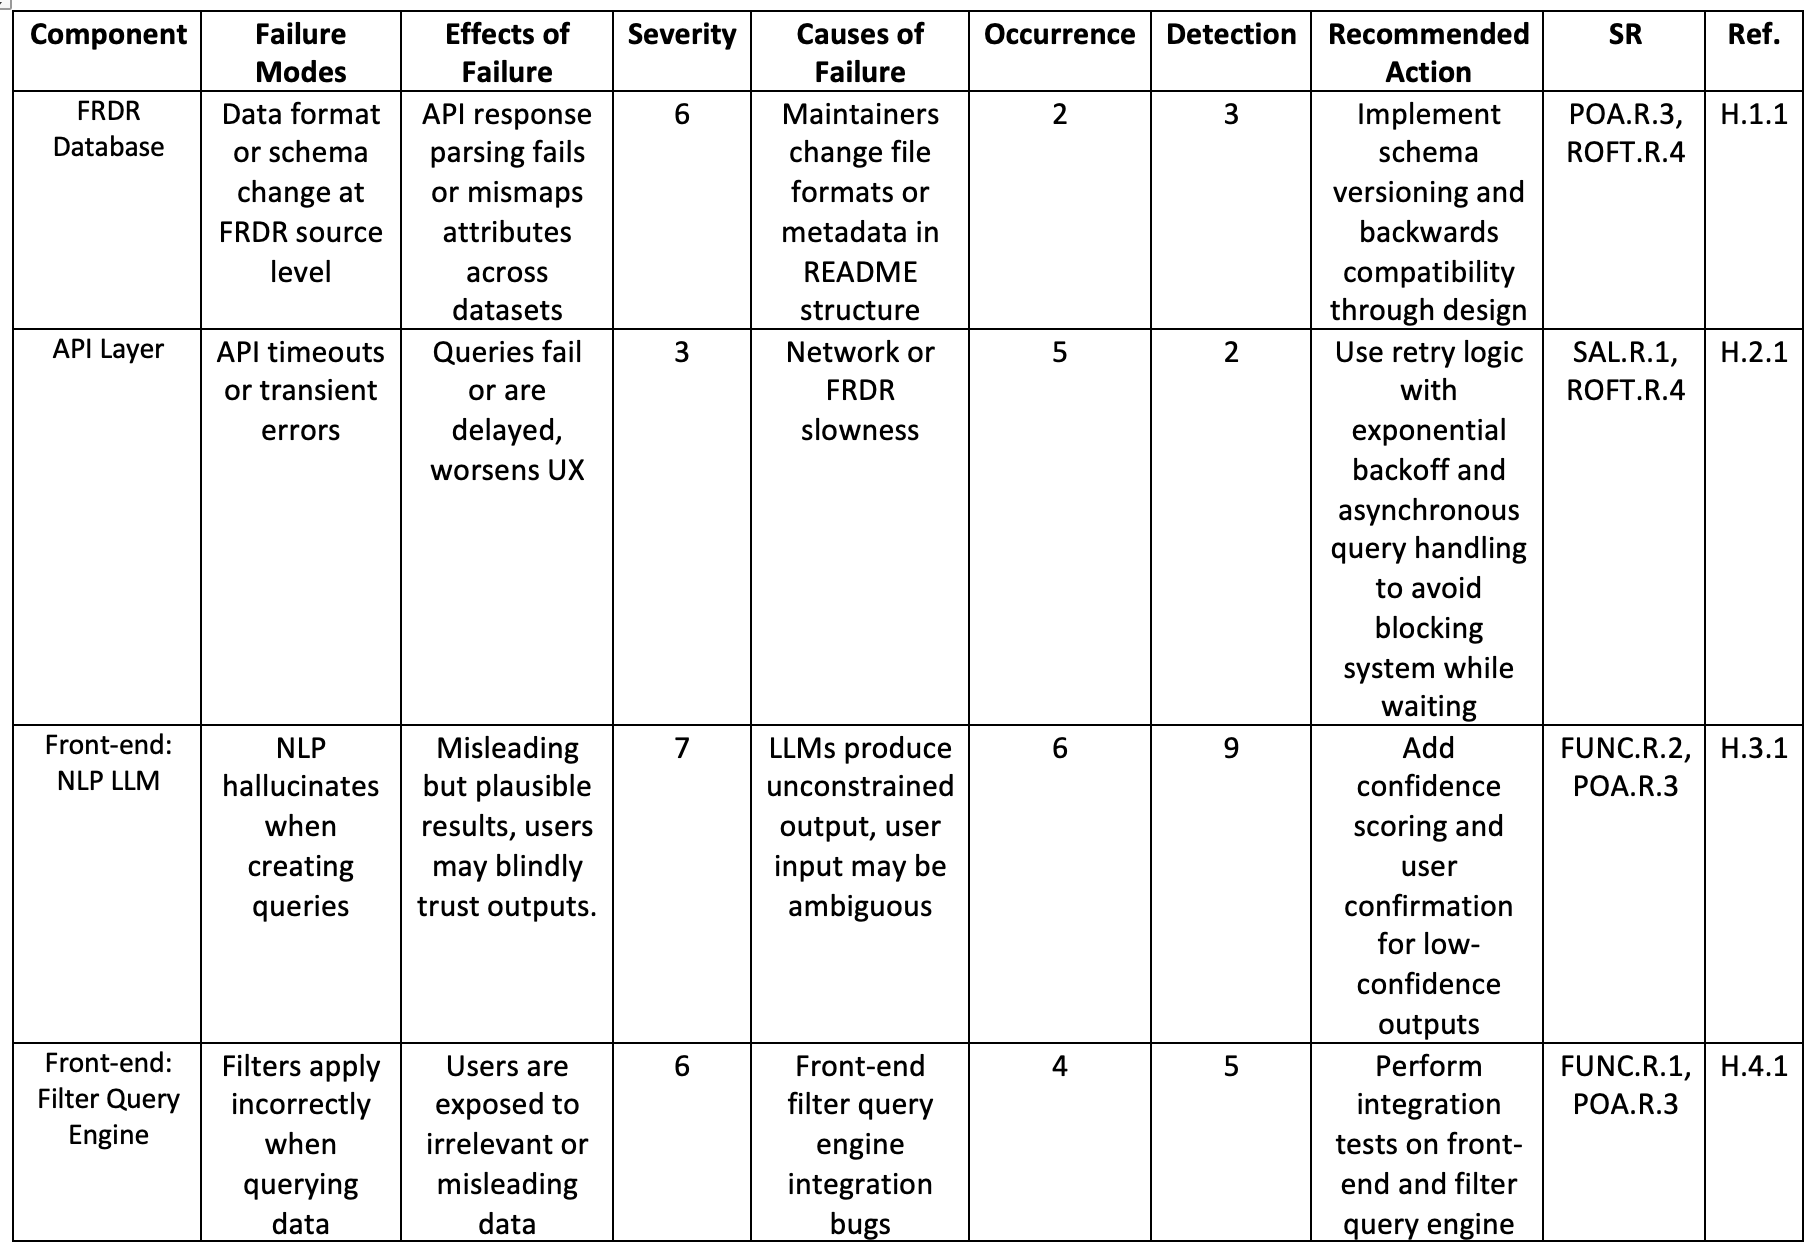
\includegraphics[width=1\textwidth]{FMEA Table 1.png}
    \caption{FMEA Table (Part 1)}
    \label{fig:TblFMEA1}
\end{figure}

\clearpage

\begin{figure}[h]
    \centering
    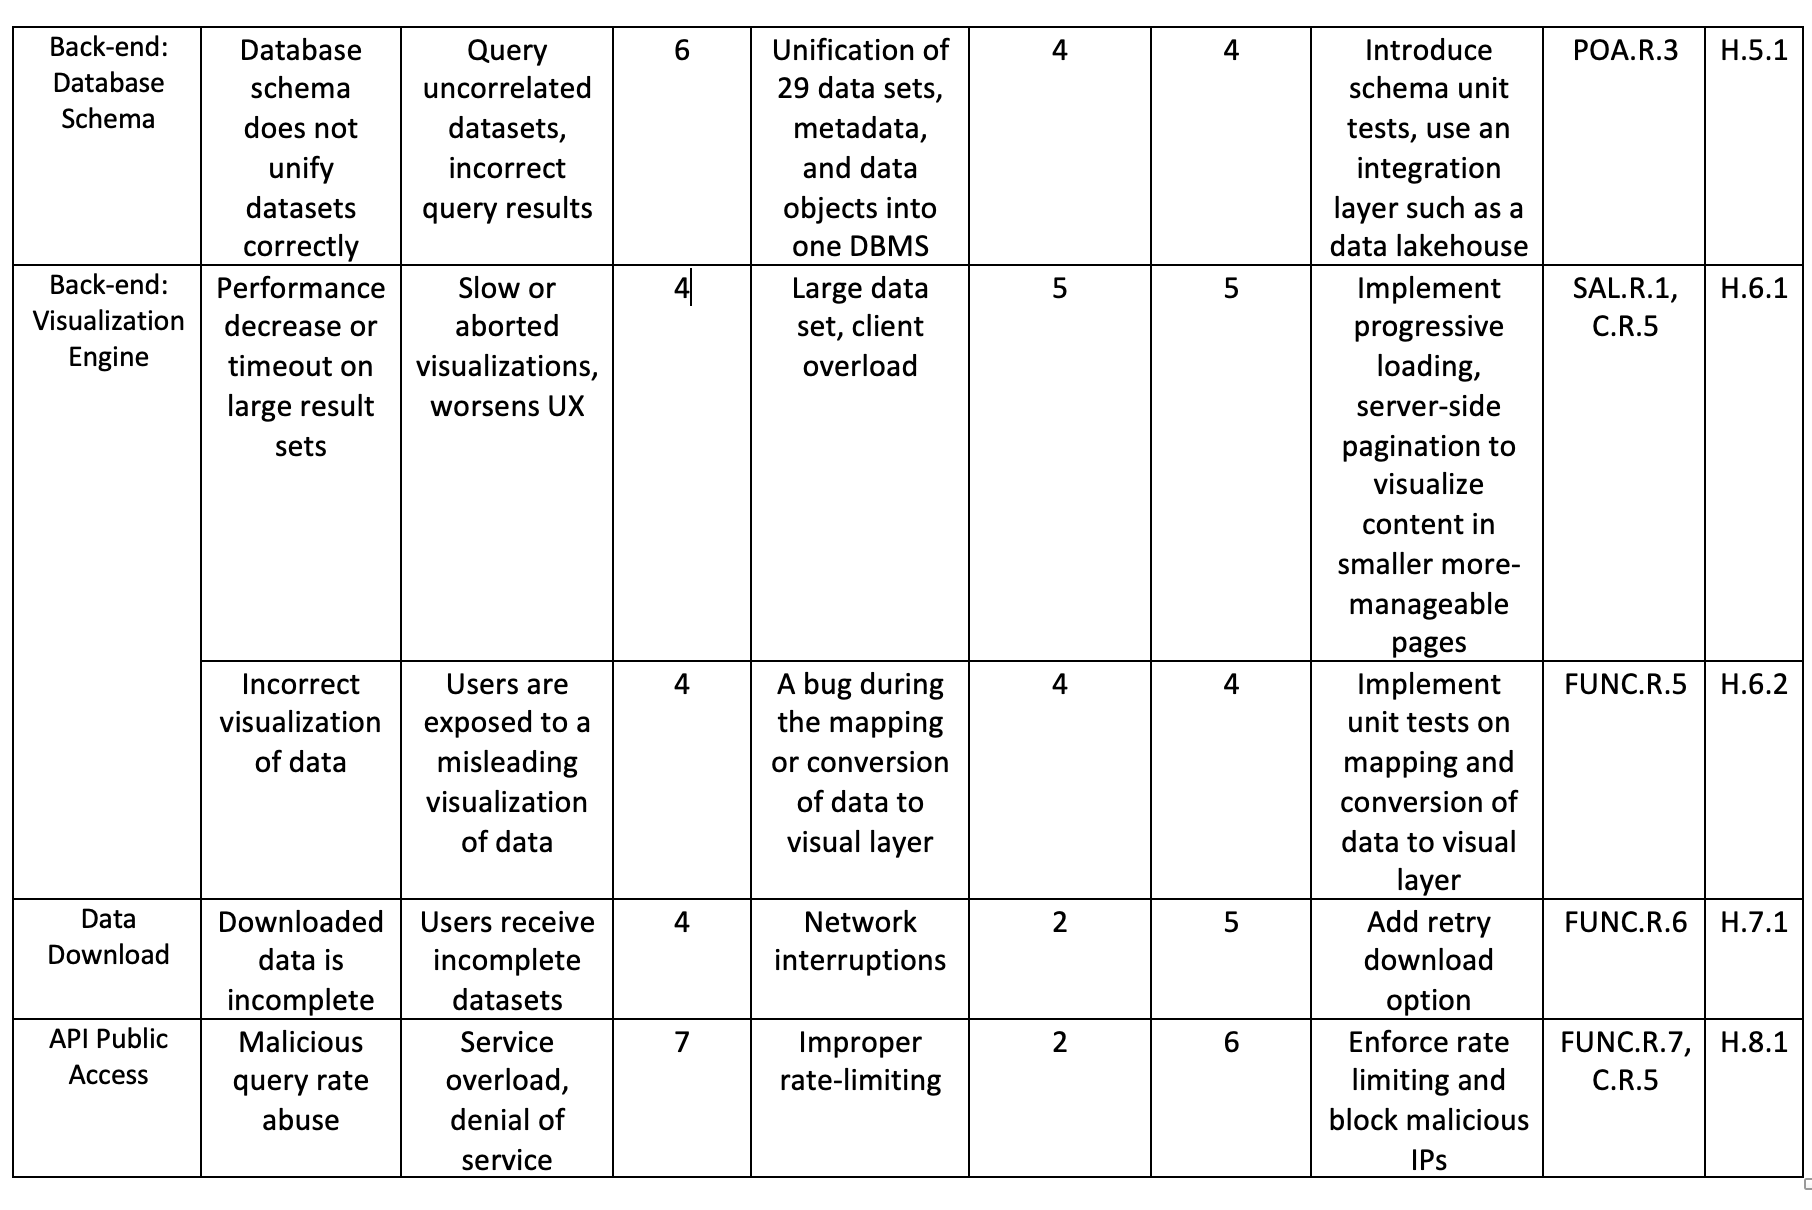
\includegraphics[width=1\textwidth]{FMEA Table 2.png}
    \caption{FMEA Table (Part 2)}
    \label{fig:TblFMEA2}
\end{figure}

\section{Safety and Security Requirements}

\subsection{Safety Requirements}
\par{The system does not directly involve physical safety or critical operations. However, to ensure data reliability and prevent unintended harm to research workflows, the following safety requirements have been identified:}
\begin{itemize}
    \item \textbf{SAF.R.1 -- Data Integrity Protection} \\
    \textbf{Description:} The system shall ensure that all query results are returned exactly as stored in the FRDR repository, without modification or corruption. \\
    \textbf{Rationale:} Prevents accidental misinterpretation of research data that could lead to invalid conclusions. \\
    \textbf{Fit Criterion:} Query results match the FRDR source files exactly, verified through checksum or metadata comparison.
    
    \item \textbf{SAF.R.2 -- Fault Isolation} \\
    \textbf{Description:} Failures in one component (e.g., NLP module) shall not compromise the operation of other system components. \\
    \textbf{Rationale:} Prevents cascading failures that could disrupt research sessions. \\
    \textbf{Fit Criterion:} The system remains operational when individual modules fail, with appropriate error messages.
    
    \item \textbf{SAF.R.3 -- Safe Handling of Large Data Sets} \\
    \textbf{Description:} The system shall prevent browsers from directly loading excessively large datasets, instead providing download or batch processing options. \\
    \textbf{Rationale:} Protects user devices from freezing or crashing during analysis. \\
    \textbf{Fit Criterion:} Queries exceeding size thresholds trigger warnings and offer alternative access methods.
\end{itemize}

\subsection{Security Requirements}
\begin{itemize}
    \item \textbf{SEC.R.1 -- Enhanced Input Validation} \\
    \textbf{Description:} All user inputs must go through validation to prevent inappropriate queries, code injection, or other malicious activity. \\
    \textbf{Rationale:} Prevents injection attacks and malformed queries from reaching backend services. \\
    \textbf{Fit Criterion:} All inputs are sanitized and penetration testing shows no injection vulnerabilities.
    
    \item \textbf{SEC.R.2 -- Access Logging} \\
    \textbf{Description:} All administrative actions, including deployment and maintenance, must be logged to provide traceability. \\
    \textbf{Rationale:} Ensures accountability and allows auditing of configuration changes. \\
    \textbf{Fit Criterion:} 100\% of administrative actions are logged with timestamps and stored securely.
    
    \item \textbf{SEC.R.3 -- Dependency Monitoring} \\
    \textbf{Description:} The system shall scan and monitor open-source frameworks, dependencies, and libraries for security vulnerabilities and update them regularly. \\
    \textbf{Rationale:} Protects against exploitation through known vulnerabilities in third-party components. \\
    \textbf{Fit Criterion:} Automated scans show no unresolved high-severity vulnerabilities older than 14 days.
    
    \item \textbf{SEC.R.4 -- Incident Documentation} \\
    \textbf{Description:} The team shall maintain documentation outlining procedures for responding to security incidents, including roles, notifications, and mitigation timelines. \\
    \textbf{Rationale:} Ensures coordinated and timely responses to potential security incidents. \\
    \textbf{Fit Criterion:} Incident response documentation exists, is reviewed regularly, and defines clear escalation steps.
    
    \item \textbf{SEC.R.5 -- Safe File Downloads} \\
    \textbf{Description:} All downloadable files shall be scanned for malware and saved with appropriate protection to safeguard user environments. \\
    \textbf{Rationale:} Prevents the distribution of malicious or corrupted files to researchers. \\
    \textbf{Fit Criterion:} All files pass malware scanning before being made available for download.
\end{itemize}


\pagebreak

\section{Roadmap}


\textbf{Scheduled for Implementation}
\par{The following safety and security requirements have been prioritized by safety and security impact and relevance to project stakeholders. }

\begin{table*}[h!]
\begin{tabularx}{\textwidth}{ X X X } 
    \textbf{ID} & \textbf{Description} & \textbf{Timing} \\
    \hline
    SAF.R.1 & Data Integrity Protection &  During Backend API integration phase   \\
    \hline 
    SAF.R.2 & Fault Isolation & During Integration Testing phase \\ 
    \hline 
    SAF.R.3 & Safe Handling  of Large Data Sets &  During backend query module implementation \\
    \hline
    SEC.R.1 & Input Validation & During frontend and API design phase \\ 
    \hline 
    SEC.R.3 & Dependency Monitoring & Immediately during development phase. \\
    \hline 
\end{tabularx}
\end{table*}



\vspace{\baselineskip}

\textbf{Deferred and Future Requirements}

\par{
The following Safety and Security requirements will not be implemented as part of the capstone due to time constraints and prioritization, however they are noted for future relevance.  
}

\begin{table*}[h!]
\begin{tabularx}{\textwidth}{ l X X } 
    \textbf{ID} & \textbf{Description} & \textbf{Justification} \\
    \hline
    SEC.R.2  & Access Logging & Low business value to client  \\
    \hline
    SEC.R.4 & Incident Documentation and response procedures & To be implemented by future maintainers of system.  \\
    \hline
        SEC.R.5 & Safe File Downloads & Out of scope for current implementation. Not a priority due to the fixed nature of FRDR data.   \\
    \hline
\end{tabularx}
\end{table*}


\newpage{}

\section*{Appendix --- Reflection}

\wss{Not required for CAS 741}

The purpose of reflection questions is to give you a chance to assess your own
learning and that of your group as a whole, and to find ways to improve in the
future. Reflection is an important part of the learning process.  Reflection is
also an essential component of a successful software development process.  

Reflections are most interesting and useful when they're honest, even if the
stories they tell are imperfect. You will be marked based on your depth of
thought and analysis, and not based on the content of the reflections
themselves. Thus, for full marks we encourage you to answer openly and honestly
and to avoid simply writing ``what you think the evaluator wants to hear.''

Please answer the following questions.  Some questions can be answered on the
team level, but where appropriate, each team member should write their own
response:


\begin{enumerate}
    \item What went well while writing this deliverable? 
    \item What pain points did you experience during this deliverable, and how
    did you resolve them?
    \item Which of your listed risks had your team thought of before this
    deliverable, and which did you think of while doing this deliverable? For
    the latter ones (ones you thought of while doing the Hazard Analysis), how
    did they come about?
    \item Other than the risk of physical harm (some projects may not have any
    appreciable risks of this form), list at least 2 other types of risk in
    software products. Why are they important to consider?
\end{enumerate}

\section{Team Reflection}
\begin{enumerate}
    \item \textbf{What went well while writing this deliverable?} \\
    One aspect that went well was our ability to clearly define and structure the requirements. We had already spoken to the client beforehand, so most of the functional requirements were straightforward to articulate. Additionally, the team collaborated efficiently, dividing the work logically at the start of the Hazard Analysis and reviewing each other's sections to maintain consistency.

    \item \textbf{What pain points did you experience during this deliverable, and how did you resolve them?} \\
    One challenge was distinguishing between functional and non-functional requirements. The client's input primarily focused on functionality and interface expectations, so we had to determine additional non-functional software-related requirements ourselves. We resolved this by holding a short internal meeting to clarify definitions and cross-check each requirement category for accuracy.

    \item \textbf{Which of your listed risks had your team thought of before this deliverable, and which did you think of while doing this deliverable? For the latter ones, how did they come about?} \\
    Before starting, we had already identified risks related to physical harm and basic security concerns. However, while completing the hazard analysis, we recognized additional risks such as data integrity issues and usability-related failures. These arose as we analyzed system interactions in more depth and considered edge cases that were not initially obvious.

    \item \textbf{Other than the risk of physical harm, list at least 2 other types of risk in software products. Why are they important to consider?} 
    \begin{itemize}
        \item \textbf{Security Risks:} These include unauthorized access, data breaches, or injection attacks. They are critical because they can compromise sensitive user information and damage system integrity.
        \item \textbf{Reliability Risks:} These involve the system failing to perform as expected under normal or stress conditions. Considering these is essential to ensure system stability and maintain user trust.
    \end{itemize}
\end{enumerate}

\end{document}
